\documentclass{article} % Document class
\usepackage{amsmath}
\usepackage{tikz}
\usepackage{pgfplots}
\usepackage{titlesec}
\title{My bs notes}
\author{Makus}
\date{\today}

\begin{document} % Begin document content
\maketitle

% \grouping{<something>} acts similar to a ToC entry for \chapter*{<something>}
%\pgfplotsset{ standard/.style={ axis line style = thick, trig format=rad, enlargelimits, axis x line=middle, axis y line=middle, enlarge x limits=0.15, enlarge y limits=0.15, every axis x label/.style={at{(current axis.right of origin)},anchor=north west}, every axis y label/.style={at={(current axis.above of origin)},anchor=south east} } }

\setcounter{secnumdepth}{4}

\titleformat{\paragraph}
{\normalfont\normalsize\bfseries}{\theparagraph}{1em}{}
\titlespacing*{\paragraph}
{0pt}{3.25ex plus 1ex minus .2ex}{1.5ex plus .2ex}

\tableofcontents

\section{Introduction}
    \begin{center}
        just random ass notes, separted by sections.
    \end{center}
    \subsection{forenotes}
    for the entire part of Computer Science, Chapter 3, the variable naming standard will be as follows:
    \begin{center}
        i is input\\ o is output
    \end{center}
    unlesss stated otherwise.
\section{math}
    \subsection{general}
        \subsubsection{bases}
        given  \begin{center}
            $n$ = base of number representation\\
            $x$ = number that is represented in base $n$,
        \end{center}
        Then $\dfrac{x}{n}$ shiftes everything in $x$ towards the left by one and $x\cdot n$ shiftes everything to the right.
        \subsubsection{logrithmic base 2}
        when taking $\log_2(1+x)$ where $0<x \leq1$, the output is approx. $x$.\\
        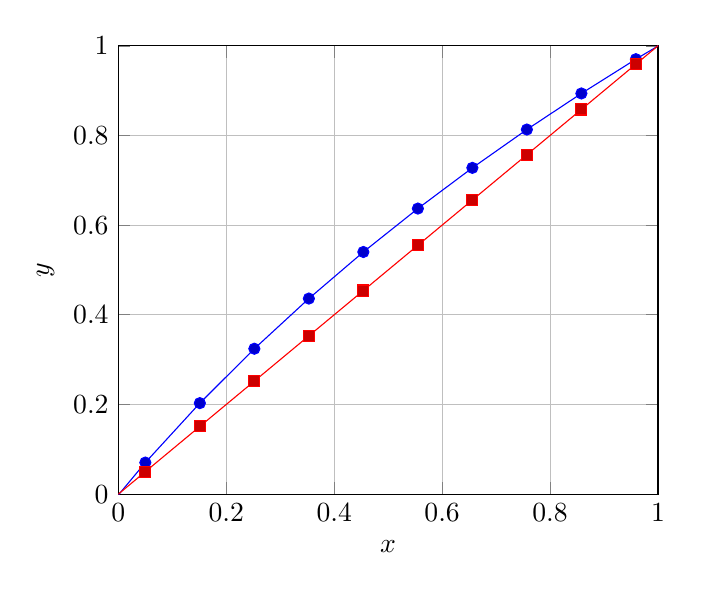
\begin{tikzpicture}
            \begin{axis}[
                xlabel={$x$},
                ylabel={$y$},
                samples=100,
                grid=major,
                xmin=0,xmax=1,
                ymin=0,ymax=1]
                \addplot{log10(x+1)/log10(2)};
                \addplot{x};
            \end{axis}
        \end{tikzpicture}
        \\but by adding $\mu$ to this, we can lower the amount of error to the average.
        to find $\mu$, we can do a mean value theorem stated in calculus portion to find $\mu$, which can be gotten from
        \begin{center}
            if $$f(x) = log_2(x+1)$$ and $$f'(c) = \dfrac{f(b)-f(a)}{b-a}$$
            \\where a=0 and b = 1, then:\\% //TODO: FIGURE OUT HOW 0.0403 IS GOTTEN TO MINIMIZE ERROR
            $$\mu = \dfrac{f(c)-c}{2}$$
            
        \end{center}
    \subsection{calculus}
        \subsubsection{Newton's iteration}
        \subsubsection{Mean Value Theorem} % (fold)
        \label{ssub:Mean Value Theorem}
            Mean Value Theorem, or MVT, states that if f(x) is continuous and differentiable within the range $a\le x \le b$, then there exists a point $c$ where $f'(c) = \dfrac{f(b)-f(a)}{b-a}$
        
        % subsubsection Mean Value Theorem (end)
\section{Computer Science}\label{Computer Science}
will be using c++ for every example
    \subsection{bit shit}
        \subsubsection{bitwise operators to stop forgetting}
            \begin{center}
                \& is and\\$|$ is or\\$\wedge$ is xor\\$\sim$ for not\\$>>$ or $<<$ for moving bits left and right respectively
            \end{center}
            \paragraph{bitwise operator quirks?}
                In C++, every number is represented in binary, or base 2. Thus if anyone were to divide a number by two, then
                \begin{verbatim}
                    x=x>>1;//shifting towards the right
                \end{verbatim}
                works the same, but is faster. it also rounds up. Conversely, if anyone were to multiply by two, then 
                \begin{verbatim}
                    x=x<<1;//shifting towards the left
                \end{verbatim}
                does the same.
        \subsubsection{IEEE 754}
            \paragraph{overview}
                This is how floats in C++ are stored. Floats are stored in 32 bit. the first bit is sign.
                The second to ninth bit is exponent, and the 10th to 32th bit is the mantissa. the exponent has
                an offset of 127, because it needs negative exponents. The mantissa, 23 bits, is the representation of the number(scientific notation).
                The equation to get from float to the final number is given by:
                \begin{equation}
                    (1+\dfrac{M}{2^{23}})\cdot2^{E-127}
                \end{equation}
            \paragraph{nitty griddy}
                The layout of this(the float) is 
                \begin{center}
                    sign bit:1 bit\\
                    exponent:1 byte(8 bits)\\
                    mantissa:23 bits\\
                \end{center}
                So if we were to follow this and try to extract exponents, we can do
                \begin{verbatim}
                    o = ((0xff<<23)&i)-127;
                \end{verbatim}
                and extracting the mantissa would be just 
                \begin{verbatim}
                    o = ((~(0xff<<23))&i);
                \end{verbatim}
                assuming the variables i and o are unsigned longs.
    \subsection{optimizations}
        \subsubsection{division}
            Since so much work has been done on addition subtraction and multiplication, the only real operation that needs change is division
            here, we will focus mostly on floats. A really easy way is to just \begin{verbatim}
                x=x/y;
            \end{verbatim}
            but in order to optimize this, we will use 
\section{physics}


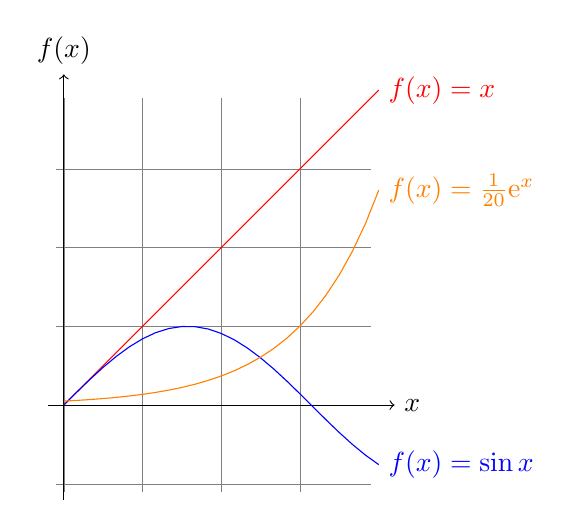
\begin{tikzpicture}[domain=0:4]
  \draw[very thin,color=gray] (-0.1,-1.1) grid (3.9,3.9);

  \draw[->] (-0.2,0) -- (4.2,0) node[right] {$x$};
  \draw[->] (0,-1.2) -- (0,4.2) node[above] {$f(x)$};

  \draw[color=red]    plot (\x,\x)             node[right] {$f(x) =x$};
  % \x r means to convert '\x' from degrees to _r_adians:
  \draw[color=blue]   plot (\x,{sin(\x r)})    node[right] {$f(x) = \sin x$};
  \draw[color=orange] plot (\x,{0.05*exp(\x)}) node[right] {$f(x) = \frac{1}{20} \mathrm e^x$};
\end{tikzpicture}
\end{document} % End document
